\documentclass{report}

% Language setting
% Replace `english' with e.g. `spanish' to change the document language
\usepackage[english]{babel}


\usepackage[a4paper,top=1.5cm,bottom=1.5cm,left=1.5cm,right=1.5cm,marginparwidth=0.75cm]{geometry}

% Useful packages
\usepackage{amsmath}
\usepackage{graphicx}
\usepackage[colorlinks=true, allcolors=blue]{hyperref}

\title{Linear Regression}
\author{Gregor Milligan}

\begin{document}
\maketitle

\begin{abstract}
This document will cover linear regression and the following topics:

\begin{itemize}
\item What is linear regression,
\item fitting a line through a set of data points
\item coding the linear regression algorithm from scratch in python
\item fitting linear regression to a housing data set using a library
\end{itemize}
\end{abstract}

\section{Introduction - What is linear regression}
Linear regression is a widely used method to estimate values such as the price of a house or value of a certain stock. The goal of linear regression is to draw a line that passes close to as many points as possible [figure 1].

"We can imagine the points as magnets lying bolted to the floor (so they can’t move). Now imagine throwing a straight metal rod on top of them. The rod will move around, but because the magnets pull it, it will eventually end up in a position of equilibrium, as close as it can to all the points." - Serrano \href{https://livebook.manning.com/book/grokking-machine-learning/chapter-3/26}{'Grokking Machine Learning'}



\begin{figure}
\centering
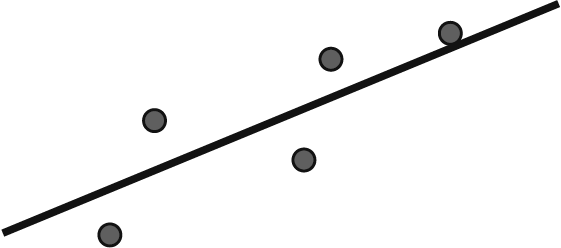
\includegraphics[width=0.3\textwidth]{lr figure 2.png}
\caption{\label{fig:lr}Linear regression.}
\end{figure}

\section{The problem: Predicting the price of a house}
A classic dataset used to introduce learners to machine learning is the \href{https://github.com/luisguiserrano/manning/blob/master/Chapter_3_Linear_Regression/Hyderabad.csv}{house price dataset}.Lets say that want to sell the house but we don't know the price, we can infer the price of a house by comparing it to other houses. To achieve this we look at features of the other houses and see how this could influence the price, for example: size , number of bedrooms, location, crime rate and so on. The goal is to create a formula for all these features that gives us the house price - or at least an accurate estimate. 

\subsection{Starting with a simple example}
We start with a simple example - we look at one feature, the number of rooms. If the house we have has 4 rooms, what would be the price? If we guess based on the table we expect it to be 300- What we did here was \emph{linear regression!}
\begin{center}
\begin{tabular}{ c c  }
 Number of rooms & Price \\ 
 1 & 150 \\
 2 & 200 \\ 
 3 & 250 \\ 
 4 & ? \\ 
 5 & 350 \\ 
 6 & 400 \\ 
 7 & 450    
\end{tabular}
\end{center}

What we did here was come up with a model represented by the formula formula $$Price = 100 + 50(Number of rooms) $$ That gave us a \emph{prediction} of price based on the \emph{feature} with is the number of rooms. The price per room is called the \emph{weight } of the corresponding feature, the base price is called the \emph{bias} of the model. 


\subsection{The elements of regression}

Lets define some of there terms in more detail:\\

FEATURES
The features of a data point are those properties that we use to make our prediction. In this case, the features are the number of rooms in the house, the crime rate, the age of the house, the size, and so on. For our case, we’ve decided on one feature: the number of rooms in the house.\\

LABELS
This is the target that we try to predict from the features. In this case, the label is the price of the house.\\

MODEL
A machine learning model is a rule, or a formula, which predicts a label from the features. In this case, the model is the equation we found for the price.\\

PREDICTION
The prediction is the output of the model. If the model says, “I think the house with four rooms is going to cost 300,” then the prediction is 300.\\

WEIGHTS
In the formula corresponding to the model, each feature is multiplied by a corresponding factor. These factors are the weights. In the previous formula, the only feature is the number of rooms, and its corresponding weight is 50. \\

BIAS
As you can see, the formula corresponding to the model has a constant that is not attached to any of the features. This constant is called the bias. In this model, the bias is 100, and it corresponds to the base price of a house. - this is constant.\\
\subsection{Multivariate Linear Regression}
What is we have more variables? We can use multivariate linear regression, rather than just predicting the house price based on the number of rooms we can image a range of variables that may impact the price of a house. For example the age of the house, the quality of the school and the size. Even though we have lots of variables our linear regression model can still work! If we have more features we just predict the price by as the sim of the feature times their corresponding weight plus a bias. The model for the price of a house could look like this: $$Price = 30(number of rooms) + 1.5(size) + 10(school quality) -2(age of the house) + 50$$

\subsection{Programming the linear regression algorithm}
The main section of this report is how we can program the linear algorithm, essentially we start by guessing where the line of best fit is, then moving this line a \emph{tiny} bit closer to the points. We repeat this process lots of times then we eventually get to the desired line.

\subsubsection{Pseduocode for the linear regression algorithm}

\boldsymbol{Inputs}: A dataset of points in the plane
\boldsymbol{Outputs}: A line the passes close to the points
Procedure:
\begin{itemize}
\item Pick a random line,
\item Repeat many times:
\item Pick a random data points
\item move the line a little closer to that points library
\item \emph{Return} the line you've obtained
\end{itemize}

\LaTeX{} is great at typesetting mathematics. Let $X_1, X_2, \ldots, X_n$ be a sequence of independent and identically distributed random variables with $\text{E}[X_i] = \mu$ and $\text{Var}[X_i] = \sigma^2 < \infty$, and let
\[S_n = \frac{X_1 + X_2 + \cdots + X_n}{n}
      = \frac{1}{n}\sum_{i}^{n} X_i\]
denote their mean. Then as $n$ approaches infinity, the random variables $\sqrt{n}(S_n - \mu)$ converge in distribution to a normal $\mathcal{N}(0, \sigma^2)$.




\end{document}